\section{Experiments}
\subsection{Public real-detection replay}
We use all nine evaluation sequences released with DMSTrack
\cite{chiu2024dmstrack} for V2V4Real~\cite{xu2023v2v4real}: 1,993 paired
frames at 10 Hz from two vehicles. Inputs are each vehicle's released
no-fusion neural detections, per-frame relative transforms, and car labels.
The detections already use a confidence cutoff of 0.20; no additional
score threshold is applied. Ground truth supplies evaluation targets only.
Births and cross-source associations use detections and posterior densities.

We evaluate planar car centers within 40 m of either sensor and inside the
annotated ego-frame rectangle $[-70.4,70.4]\times[-40,40]$ m. A 3 m disk
around each sensor excludes the sensing platforms, whose bodies are masked
by detector preprocessing but present in the labels. The same domain applies
to detections, reported estimates, and truth, and to the likelihood and
absence tests. The 40 m crop defines a conservative modeled FoV, not an
occlusion map. Detections are already expressed in the current ego frame;
the second vehicle's transform locates its sensor. The relative-frame
constant-velocity model lacks ego-motion compensation.

The shared LBP-LMB backend moment-projects each Bernoulli to one Gaussian,
including association uncertainty. It uses $\Delta t=0.1$ s, survival
0.99, white-acceleration intensity 25 m$^2$/s$^3$, observation covariance
$I_2$ m$^2$, nominal in-domain $p_D=0.9$, Poisson clutter mean three per
scan, and pruning at $r\leq0.001$. Each source independently creates a
birth at every previous-scan detection with $r_B=0.01$, zero velocity,
and covariance $\operatorname{diag}(16,16,225,225)$. These fixed model
assumptions are shared by all methods. ER retains $\rho=0.25,\lambda=5$ s.

Each sequence is replayed with reliable links and with emulated intermittent
links: independent directed loss of 0.1 plus a bidirectional outage over the
middle 20\% of scans. All methods share the delivered graph and one packet
opportunity per direction per scan. Received density pairs use equal weights.
This is an exploratory two-dimensional fusion evaluation: preflight domain
and resource corrections preceded the complete cohort. It is not the
official three-dimensional benchmark or a reproduction of DMSTrack's
learned tracker.

\subsection{Mechanism case studies}
\begin{figure*}[t]
 \centering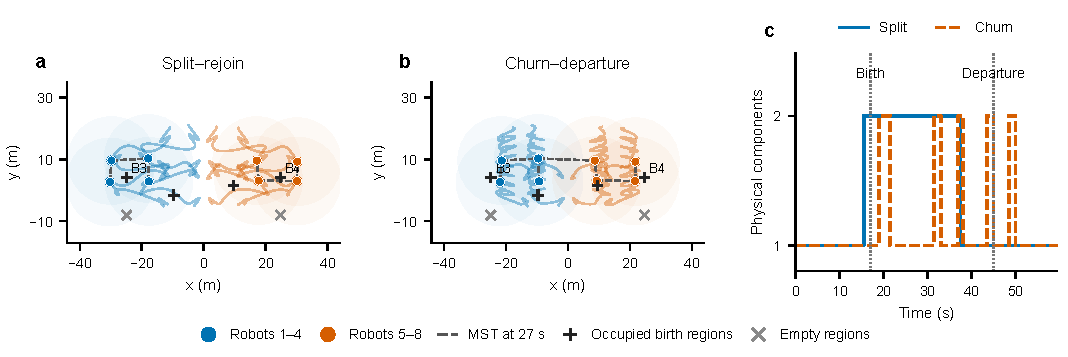
\includegraphics[width=\textwidth]{figures/scene.pdf}
 \caption{Mechanism case studies. Thin curves are robot paths; circles and
 dashed tree edges show the state at 27 s. Light disks denote 14 m FoVs.
 Crosses mark candidate birth regions; the two lower regions remain empty.
 The split and churn scenarios create different contact histories, with
 target departure at 45 s in the churn scenario.}
 \label{fig:scene}
\end{figure*}
Eight simulated robots follow two smooth patrol families for 120 frames
at $\Delta t=0.5$ s. Their maximum speed is below $3$ m/s and acceleration
below $2.1$ m/s$^2$. Radio range is $24$ m and circular sensing range is
$14$ m. The fixed paths induce connected and two-component periods
(Fig.~\ref{fig:scene}).
All targets use a constant-velocity state
with independent per-step acceleration standard deviation $0.016$ m/s$^2$.
The filter uses a continuous white-acceleration covariance with intensity
$0.0128$ and survival probability $0.995$. Within FoV, detection probability is
$0.9$ and Cartesian observation noise has standard deviation $0.4$ m.
Poisson clutter has mean one per robot per frame and is uniform over a
fixed $104\times80$ m rectangle. Local pruning discards
existence at or below $0.01$; belief propagation uses tolerance $10^{-6}$
and at most 1,000 iterations. All methods share these settings.

The \emph{split--rejoin} scene has two initial targets and two targets born
at frame 35 while the teams are separated. The \emph{churn--departure} scene
uses repeated contact changes and removes one late target after frame 90;
the filters receive no departure notification. In the \emph{no-new} control,
only the two initial targets exist, although identical later birth priors
are still offered. Six fixed candidate regions have prior existence $0.1$,
position standard deviation $3.2$ m, and velocity standard deviation
$0.2$ m/s. Regions 1--2 are activated at frame 1 and regions 3--6 at frame
35. Regions 5--6 remain empty in every scene. The filters receive the
candidate birth schedule and priors.

Each scenario uses twenty Monte Carlo trials. In each trial, every robot
receives an independent constant path offset drawn uniformly from
$[-0.6,0.6]^2$ m, and the communication components and trees are recomputed.
The offsets vary the layout and contacts while preserving speed and
acceleration. Target trajectories, detections, clutter, and directed
link-loss draws are paired across methods. Directed packet loss is $0.1$.

\subsection{External methods, controls, and ablations}
\emph{TC-OSPA$^2$} uses the unchanged author kinematic matching and
multi-neighbor fusion functions~\cite{nguyen2021tc}, with windows of five
and ten scans, matching order one and cutoff 12 m. Its input is the shared
Local backend's track estimates with independent node label namespaces.
Following the author's architecture, fused tracks do not feed back into
local densities. Both kinematic fusion stages are local computations on
communicated histories. We evaluate set estimates; network-wide reporting
label reconciliation is excluded. This adapts the published strategy to our
local backend rather than reproducing its original filtering experiment.

\emph{MIL-AM} implements the public Gao author manuscript's augmented
label assignment and common/exclusive label-subspace LMB-MIL
\cite{gao2019milpreprint}. For Gaussian inputs, matching uses its symmetric
KL cost, with unmatched cost 50 per side. Common labels use arithmetic
existence pooling and existence-weighted spatial mixtures; exclusive labels
retain their source density. The same label alignment is applied to ER and
its no-age ablation. Spatial mixtures are moment-projected in the real
replay. This implementation is tied to the public manuscript; equivalence
to the complete TAES 2022 version~\cite{gao2022differentfov} is not established.

\emph{Local} runs without communication. \emph{FoV} uses FoV-based absence
censors. \emph{ER w/o age} adds observation-history qualification and
omits the age factor. \emph{Age-all} applies direct-age weights to both
spatial and existence pooling without history-based qualification.
\emph{ER (both)} adds this qualification, separating placement of the age
factor from input selection. \emph{ER} uses the same qualification with
age in existence alone. \emph{Confirmed ER} adds the two-hit gate.

The \emph{MIL-Z} control uses constrained LMB MIL,
$r=\sum_jw_jr_j$ and $p=\sum_jw_jr_jp_j/r$, with zero existence for absent
labels~\cite{gao2020mil}. \emph{MIL-S} specializes label-subspace MIL
\cite{gao2020mil,gao2022differentfov} to the shared-label setting: for each
subspace defined by a source-membership pattern, weights are renormalized
over represented sources before applying the same pooling formula. Both
MIL controls use the shared birth keys for label alignment and retain
untouched represented priors. Their Gaussian-mixture unions are reduced
to the common component cap.

MIL-AM is evaluated on the real replay with independent births. The
shared-label MIL-Z/S controls and the additional mechanism ablations are
evaluated in the robot case studies.

\subsection{Metrics and uncertainty}
We report position OSPA with order $2$ and cutoff $12$ m
\cite{schuhmacher2008ospa}, cardinality absolute error, and GOSPA with
$p=2,c=12$ m,$\alpha=2$~\cite{gospa2017}. Localization, missed-target,
and false-target GOSPA components are reported as \emph{squared costs}
in m$^2$. In the case studies, all extant targets are scored at every robot, including during
disconnection. The scores therefore measure team-wide information coverage
as well as local tracking.

For localization comparisons, assignments are computed separately for each
method and matched errors are pooled only on robot--time--truth triples
matched within the cutoff by both methods. We report the resulting RMSE
and common-support size; unmatched targets contribute to OSPA/GOSPA.
Departure false cost uses frames 91--120. Reunion OSPA uses the next ten
frames, truncated at a further disconnection. For opposite-subteam robots,
acquisition is defined geometrically as the first of three consecutive
assignments within 2 m of a late target, censored at that target's departure
or the trial end.

We use 10,000 paired bootstrap resamples for 95\% percentile intervals.
The unit is a complete trial for the case studies and a complete sequence
for real data; sequence means receive equal weight. Frames and robots are
not independent replicates. With only nine potentially related driving
sequences, real-data intervals are descriptive.
